% !TeX root = RJwrapper.tex
\title{Editorial}
\author{by Catherine Hurley}

\maketitle


On behalf of the editorial board, I am pleased to present Volume 14 Issue 3 of the R Journal.

\noindent Our incoming editor-in-chief for 2023 Simon Urbanek has been successful in seeking funding from the R Consortium. The project will provide a web-based front-end for managing the R Journal submission and review process.

\noindent Behind the scenes, several people assist with the journal operations. Mitchell O'Hara-Wild continues to work on infrastructure, and thanks to this work, producing a new issue is far more straightforward. H. Sherry Zhang continues to develop the \CRANpkg{rjtools} package under the direction of Professor Dianne Cook. This package, recently available from CRAN assists in producing RMarkdown articles in the R Journal format. In addition, articles in this issue have been carefully copy edited by Hannah Comiskey.

\hypertarget{in-this-issue}{%
\subsection{In this issue}\label{in-this-issue}}

News from the CRAN and Bioconductor are included in this issue.

\noindent This issue features 18 contributed research articles the majority of which relate to R packages
on a diverse range of topics. All packages are available on CRAN. The most common article keywords in this issue are

\begin{center}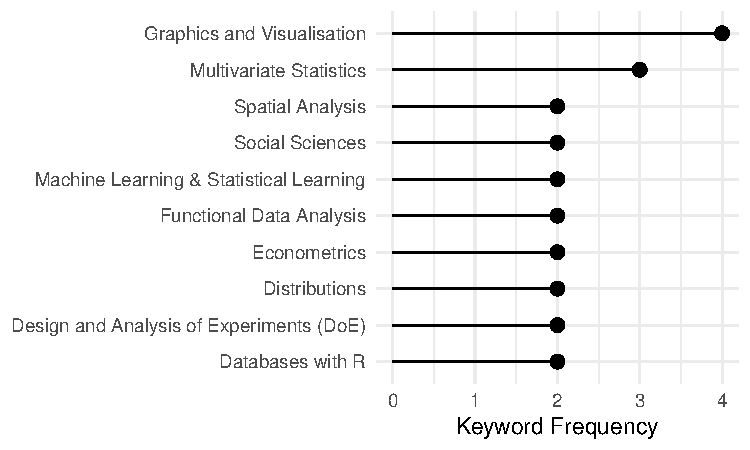
\includegraphics[width=0.5\linewidth]{figs/keywords-1} \end{center}

\noindent For the first time, we give times from submission to article acceptabce for an issue. Median times are just under a year, which is consistent other issues over the last few years.

\begin{center}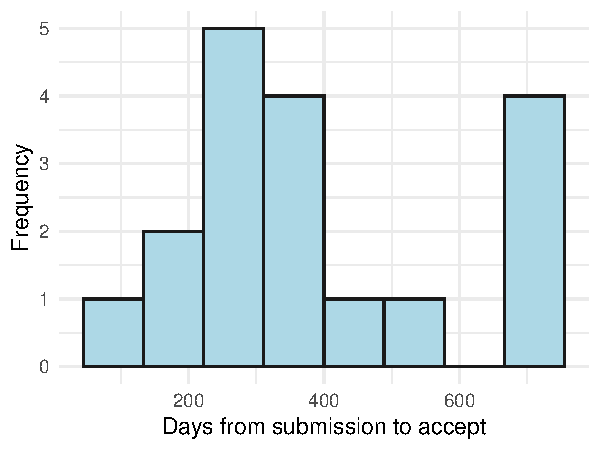
\includegraphics[width=0.5\linewidth]{figs/days-1} \end{center}


\address{%
Catherine Hurley\\
Maynooth University\\%
\\
%
\url{https://journal.r-project.org}\\%
%
\href{mailto:r-journal@r-project.org}{\nolinkurl{r-journal@r-project.org}}%
}
